\documentclass{article}
\usepackage{tikz}
\usetikzlibrary{arrows.meta, positioning}

\begin{document}

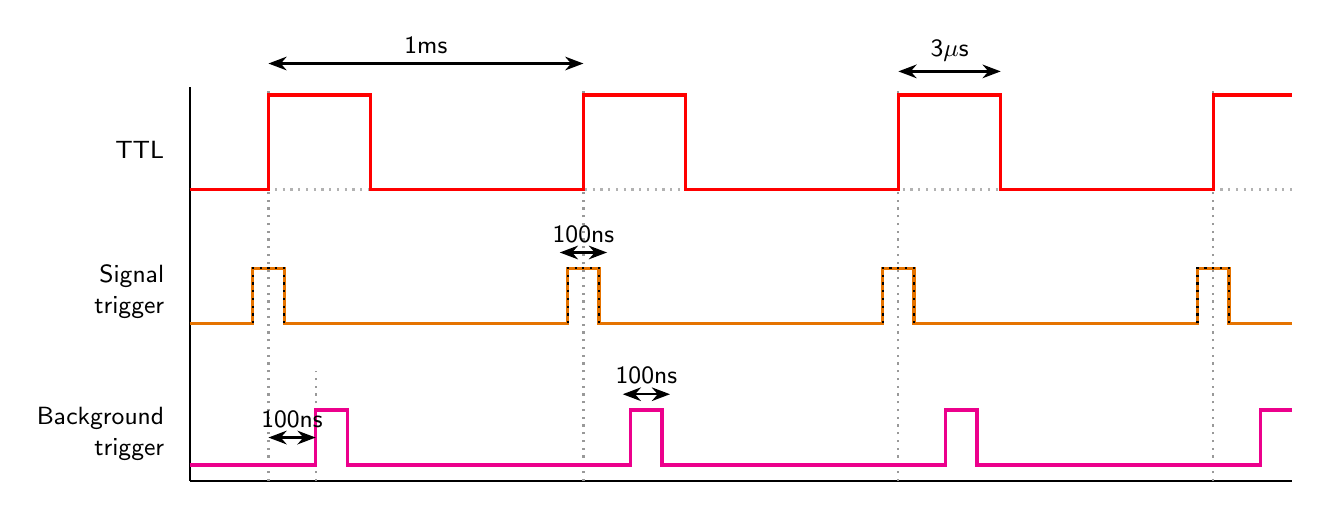
\begin{tikzpicture}[
    >=Stealth,
    font=\sffamily\small,
    axis/.style={thick},
    dottedline/.style={dotted, thick, gray!80},
    dim/.style={<->, >=Stealth, thick}
]

    % Define track vertical offsets
    \def\yTTL{3.5}
    \def\ySig{1.8}
    \def\yBg{0.0}

    % 1. Vertical Axis Baseline
    \draw[axis] (-0.5, -0.2) -- (-0.5, 4.8);

    % Horizontal Axis Baseline
    \draw[axis] (-0.5, -0.2) -- (13.5, -0.2);

    % Track Labels on the Left
    \node[left, align=right] at (-0.7, \yTTL + 0.5) {TTL};
    \node[left, align=right] at (-0.7, \ySig + 0.4) {Signal\\trigger};
    \node[left, align=right] at (-0.7, \yBg + 0.4) {Background\\trigger};

    % -------------------------------------------------------------
    % Dotted Vertical Alignment Lines & Key Coordinates
    % (Pulse positions across four repeating periods)
    % -------------------------------------------------------------
    \coordinate (t0) at (0.5, 0);
    \coordinate (t1) at (4.5, 0);
    \coordinate (t2) at (8.5, 0);
    \coordinate (t3) at (12.5, 0);

    \foreach \x in {0.5, 4.5, 8.5, 12.5} {
        \draw[dottedline] (\x, -0.2) -- (\x, 4.8);
    }

    % Additional dotted lines for background delay alignment
    \draw[dottedline] (1.1, -0.2) -- (1.1, 1.2);

    % -------------------------------------------------------------
    % 1. TTL Waveform (Red)
    % -------------------------------------------------------------
    \draw[dotted, thick, gray!60] (-0.5, \yTTL) -- (13.5, \yTTL); % Base level ref line
    \draw[red, line width=1.2pt] 
        (-0.5, \yTTL) -- (0.5, \yTTL) 
        -- (0.5, \yTTL+1.2) -- (1.8, \yTTL+1.2) -- (1.8, \yTTL) 
        -- (4.5, \yTTL) 
        -- (4.5, \yTTL+1.2) -- (5.8, \yTTL+1.2) -- (5.8, \yTTL) 
        -- (8.5, \yTTL) 
        -- (8.5, \yTTL+1.2) -- (9.8, \yTTL+1.2) -- (9.8, \yTTL) 
        -- (12.5, \yTTL) 
        -- (12.5, \yTTL+1.2) -- (13.5, \yTTL+1.2);

    % -------------------------------------------------------------
    % 2. Signal Trigger Waveform (Orange / Gold)
    % -------------------------------------------------------------
    \draw[orange!90!black, line width=1.2pt] 
        (-0.5, \ySig) -- (0.3, \ySig) 
        -- (0.3, \ySig+0.7) -- (0.7, \ySig+0.7) -- (0.7, \ySig) 
        -- (4.3, \ySig) 
        -- (4.3, \ySig+0.7) -- (4.7, \ySig+0.7) -- (4.7, \ySig) 
        -- (8.3, \ySig) 
        -- (8.3, \ySig+0.7) -- (8.7, \ySig+0.7) -- (8.7, \ySig) 
        -- (12.3, \ySig) 
        -- (12.3, \ySig+0.7) -- (12.7, \ySig+0.7) -- (12.7, \ySig) 
        -- (13.5, \ySig);

    % Dotted outline for signal pulses
    \draw[dotted, thick] (0.3, \ySig) -- (0.3, \ySig+0.7) -- (0.7, \ySig+0.7) -- (0.7, \ySig);
    \draw[dotted, thick] (4.3, \ySig) -- (4.3, \ySig+0.7) -- (4.7, \ySig+0.7) -- (4.7, \ySig);
    \draw[dotted, thick] (8.3, \ySig) -- (8.3, \ySig+0.7) -- (8.7, \ySig+0.7) -- (8.7, \ySig);
    \draw[dotted, thick] (12.3, \ySig) -- (12.3, \ySig+0.7) -- (12.7, \ySig+0.7) -- (12.7, \ySig);

    % -------------------------------------------------------------
    % 3. Background Trigger Waveform (Magenta)
    % -------------------------------------------------------------
    \draw[magenta, line width=1.2pt] 
        (-0.5, \yBg) -- (1.1, \yBg) 
        -- (1.1, \yBg+0.7) -- (1.5, \yBg+0.7) -- (1.5, \yBg) 
        -- (5.1, \yBg) 
        -- (5.1, \yBg+0.7) -- (5.5, \yBg+0.7) -- (5.5, \yBg) 
        -- (9.1, \yBg) 
        -- (9.1, \yBg+0.7) -- (9.5, \yBg+0.7) -- (9.5, \yBg) 
        -- (13.1, \yBg) 
        -- (13.1, \yBg+0.7) -- (13.5, \yBg+0.7);

    % -------------------------------------------------------------
    % Dimensions & Annotations
    % -------------------------------------------------------------

    % 1 ms Period Annotation at top
    \draw[dim] (0.5, \yTTL + 1.6) -- (4.5, \yTTL + 1.6) 
        node[midway, above] {1ms};

    % 3 us Width Annotation on TTL pulse
    \draw[dim] (8.5, \yTTL + 1.5) -- (9.8, \yTTL + 1.5) 
        node[midway, above] {3$\mu$s};

    % 100ns Pulse Width on Signal Trigger
    \draw[dim] (4.2, \ySig + 0.9) -- (4.8, \ySig + 0.9) 
        node[midway, above] {100ns};

    % 100ns Delay Annotation between TTL & Background pulse
    \draw[dim] (0.5, \yBg + 0.35) -- (1.1, \yBg + 0.35) 
        node[midway, above] {100ns};

    % 100ns Pulse Width on Background Trigger
    \draw[dim] (5.0, \yBg + 0.9) -- (5.6, \yBg + 0.9) 
        node[midway, above] {100ns};

\end{tikzpicture}

\end{document}
